\documentclass[pdflatex,sn-basic]{sn-jnl}
\usepackage[T1]{fontenc}
\usepackage[utf8]{inputenc}
\DeclareUnicodeCharacter{2212}{\ensuremath{-}}
\usepackage{lmodern,amsmath,amssymb,booktabs,tabularx,graphicx,microtype,xurl}
\usepackage{enumitem}
\setlist{nosep}
\providecommand{\tightlist}{\setlength{\itemsep}{0pt}\setlength{\parskip}{0pt}}
\setlength{\emergencystretch}{2em}
\raggedbottom
\begin{document}
\title[Approval Scope and Recovery in Agentic Software]{The Review--Execution Gap in Agentic Software: Approval Scope and Recovery}
\author[1]{Liang Hanghao}
\author[1]{Xuan Wentao}
\author[1]{Chen Qile}
\author*[1]{Peng Peng}\email{hnu16pp@hnu.edu.cn}
\affil[1]{\orgdiv{College of Computer Science and Electronic Engineering},
\orgname{Hunan University},
\orgaddress{\city{Changsha}, \postcode{410082}, \country{China}}}
\abstract{Human review constrains what agentic workflows may execute, yet agents can regenerate or resume proposed updates after approval. A correct final value alone cannot establish that the executed candidate was covered by the review. We investigate how an application's declared approval scope governs admission at a durable execution boundary and how agents continue after an instance mismatch. We develop a four-role correction contract linking the machine proposal, authorized correction, reviewed candidate, and persisted transition. For context- and instance-bound admission, we hold the shared authority, freshness, atomicity, and provenance obligations fixed; controlled comparator cases additionally examine content binding and external-reference changes. Relational and event-journal implementations and bounded formal checks assess the contract's persistence obligations. A configured ToolGate adaptation tests implementability, while pinned SDK probes separately examine reviewed-argument consumption and continuation routes. In a reduced agent host with a deterministic reviewer, 32 delivered identity-only substitution pairs span 16 task definitions. Context binding admits every substitute, and 30 context continuations complete. Instance binding rejects every substitution; all 32 instance-bound continuations recover, with 24 reusing the reviewed candidate and eight obtaining fresh authorization. Archived states and model inputs establish that reuse remained available and visible in all 32 episodes. These continuations incur additional tool calls, without an established task-completion advantage. Approval scope therefore defines admissible reuse, while agents' subsequent choices determine recovery routes and their interaction costs. The authorization boundary and the continuation it enables must be designed and evaluated together.}
\keywords{Agentic software, Human review, Runtime enforcement, Authorization, Provenance, Empirical evaluation}
\maketitle
\begin{figure}[t]
\centering
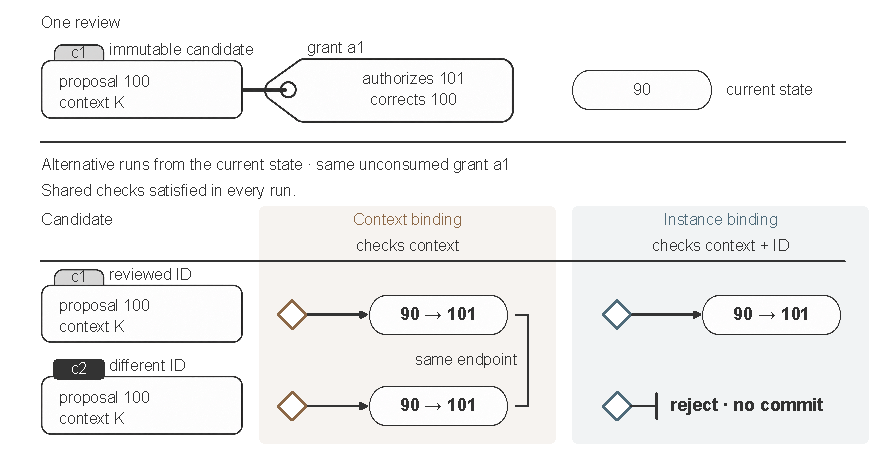
\includegraphics[width=\linewidth]{figures/fig1-review-execution-gap.pdf}
\caption{Equal endpoints do not identify the reviewed instance. Candidate c1 proposes 100; grant a1 authorizes the correction 101 for c1. Candidate c2 retains the same context $K$ with a different identifier. Alternative paths start from state 90 with a1 unconsumed and all shared checks satisfied: context binding admits either candidate, whereas instance binding admits only c1. Diamonds are checks, capsules are states/transitions, and the stop bar means no commit. A matching new grant may authorize c2. The four roles are proposal 100, correction 101, reviewed c1 and executed transition $90\to101$. Conceptual construction; AI-generated object glyphs are disclosed below}
\label{fig:gap}
\end{figure}

\section{Introduction}\label{introduction}

Human approval depends on understanding a proposed change \citep{bacchelli2013review} and determining whether that decision still applies at execution. Established workflows make this applicability configurable: Gerrit controls vote copying across patch sets and submit requirements \citep{gerrit-copy-condition,gerrit-submit-requirements}; GitLab distinguishes deployment approval from merge-request approval reset \citep{gitlab-deployment-approval,gitlab-approvals}. Each approval object---revision, change or deployment instance---determines which replacements remain covered.

In agentic software, a language-model controller selects tool actions from execution feedback \citep{wang2026agr}, while approval middleware can pause, edit, reject and resume a call \citep{langchain-hitl}. A controller may regenerate or retrieve a candidate after review. Even if its content and intended effect are unchanged, the application must decide whether the earlier business grant covers that candidate.

Consider an agent-generated release-change record c1 that proposes replacing 90 with 100. A reviewer authorizes the correction 101. Before persistence the workflow produces c2 with the same proposal, evidence, target and expected predecessor. Executing c2 produces the same final value as executing c1, but whether the earlier approval authorizes c2 depends on the application's approval scope: a context- or content-scoped policy may permit the replacement, while an instance-scoped policy requires the reviewed record or a new matching authorization. The final state alone cannot distinguish these authorization histories. We call the unresolved relationship between the reviewed object and the executed operation the \textbf{review--execution gap}.

The gap has two connected parts: enforcing approval scope together with value correctness, predecessor freshness and provenance, and enabling continuation after rejection. An agent may reuse the reviewed candidate, obtain new authorization or stop when no valid route remains. These routes have different costs even when they reach the same business state. GitLab's deployment-specific approvals illustrate an operational instance rule \citep{gitlab-deployment-approval}; the interface alone does not determine an agent's continuation or its cost.

Several mechanisms keep authorization valid up to execution: reconstruction-aware authorization \citep{zhu2026resa}, guarded commits with pinned policy and edit hashes \citep{bindschaedler2026guarded}, analyses of reviewed-call substitution \citep{kumar2026loopjacking,wang2026approval}, and repair obligations or commit-time validity certificates \citep{wang2026acg,qi2026revise}. Each addresses a different moment between review and effect. What remains open is how approval scope changes both admissible execution and autonomous continuation under shared correction and persistence obligations. Enforcement determines which replacements execute; continuation shows what a rejection costs.

We ask three questions. \textbf{RQ1}: which candidate replacements can legitimately reuse an existing approval under context-, content- and instance-based policies? \textbf{RQ2}: how can the selected approval relationship be checked together with authorized corrections, current predecessors, atomic transitions and field-level provenance? \textbf{RQ3}: after an instance mismatch, which legal recovery routes do agents take, and what do those routes cost?

We make three connected contributions.

\begin{enumerate}
\item \textbf{A unified comparison of correction and approval scope.} We formulate a four-role contract connecting the machine proposal, the authorized correction, the reviewed candidate and the persisted transition. Holding value, freshness, provenance and atomicity obligations fixed, we characterize how approval scope changes admissibility, and nine constructed cases separate omitted-field changes, equivalent re-materialization and mutable external references, identifying which protections follow from the binding rule and which require a separate consumption check.
\item \textbf{Cross-layer validation of review-to-execution continuity.} Relational and event-journal stores assess the durable relations, checked by an independent oracle and bounded formal analysis. A ToolGate adaptation tests whether an existing gate can carry the obligations through its extension interface. Three pinned SDKs then examine what a resumed call executes: a matching native call identifier need not preserve the reviewed arguments, although these probes do not test contract enforcement.
\item \textbf{An empirical account of recovery under explicit approval rules.} At controlled handoffs in a reduced host with a deterministic reviewer, 32 delivered identity-only substitutions from 16 task definitions are admitted under context binding and rejected under instance binding. All 32 rejected continuations recover, but agents choose different legal routes: 24 reuse the reviewed candidate and eight obtain fresh authorization. Archival reconstruction establishes that the reviewed candidate and its grant were available and visible in the saved model input in all 32 episodes, including the eight that reauthorized. We separate recovery from later confirmation and renewed authorization requests and report their call and elapsed-time costs.
\end{enumerate}

Table~\ref{tab:evidence-map} maps each question to its evidence. The agent comparison holds retained content fixed ($K=R$); it measures the behavioral cost of an instance requirement.

\begin{table}[bp]
\caption{Research questions, evidence and the claim each layer supports. Controlled conditions, trajectories and historical records are distinct units.}\label{tab:evidence-map}
\centering\small
\begin{tabularx}{\textwidth}{@{}>{\raggedright\arraybackslash}p{0.15\textwidth}>{\raggedright\arraybackslash}p{0.39\textwidth}>{\raggedright\arraybackslash}X@{}}
\toprule
Question & Evidence & Supported claim \\
\midrule
RQ1 & Local specification and nine constructed cases & Distinguish approval scope under stated storage and comparator assumptions (Sections~\ref{what-endpoint-correctness-cannot-establish},~\ref{binding-scope-and-native-defaults}). \\
RQ2 & 165 controlled cases per mechanism (context journal; exact journal and relational reference); 24 scripted public routes per implementation & Validate durable relations and framework extension feasibility (Section~\ref{realization-and-external-comparison}). \\
RQ2 & 16 native interrupt conditions; 10 scripted integration conditions; 504 reviewed-argument cells; 54 route-ablation cells; 16 substitution cells & Distinguish native resume routing and application grant enforcement (Section~\ref{binding-scope-and-native-defaults}; Online Resource 2, A14, A17). \\
RQ3 & 32 delivered identity-handoff pairs; archived state and visible-input reconstruction & Observe recovery routes and agent-side costs across 16 task definitions (Section~\ref{two-routes-to-accountable-recovery}). \\
RQ3 & 12 exploratory feedback pairs and 24 rule trajectories & Test continuation under three permission states; compare path labels with the same facts (Section~\ref{feedback-sensitivity}). \\
\bottomrule
\end{tabularx}
\end{table}

\section{Related Work}\label{related-work}

\subsection{What existing mechanisms bind}\label{existing-binding-and-enforcement-mechanisms}

Table~\ref{tab:related} compares binding objects, mismatch handling and check points. Configurable code-review approval \citep{gerrit-copy-condition,gitlab-approvals} motivates our comparison for corrected agent state and subsequent continuation.

\begin{table}[tbp]
\caption{Binding, mismatch handling and evidence in the cited sources. The two attack analyses describe failure paths; their check points are observation points.}\label{tab:related}
\centering\footnotesize
\setlength{\tabcolsep}{2.5pt}
\renewcommand{\arraystretch}{1.05}
\begin{tabularx}{\textwidth}{@{}>{\hsize=1.05\hsize\raggedright\arraybackslash}X>{\hsize=1.0\hsize\raggedright\arraybackslash}X>{\hsize=1.05\hsize\raggedright\arraybackslash}X>{\hsize=.75\hsize\raggedright\arraybackslash}X>{\hsize=1.15\hsize\raggedright\arraybackslash}X@{}}
\toprule
Mechanism & Binding object & Mismatch handling & Check point & Evaluation form \\
\midrule
LangChain HITL \citep{langchain-hitl} & Interrupted tool call & Reviewer may edit/reject, then resume & Before tool execution & Interface documentation \\
ReSA \citep{zhu2026resa} & Exact/scoped grant; consumed versions & Derive repair obligations & Reconstruction to local sink & Authored graphs; installed-control checks \\
Guarded Commits \citep{bindschaedler2026guarded} & Artifact, policy; edit hashes & Fresh authorization or review & Commit & Public-trace replay; synthetic DAGs \\
Cordon \citep{cordon} & Task, lineage, staged effects & Abort, rollback, compensation & Commit or effect release & Agent workflows; scripted rollback/resume \\
Continuity Kernel \citep{continuity-kernel} & Proposal ID; sealed successor & Reject, quarantine or defer; new-ID retry & Atomic activation & Bounded model exploration \\
Commit-time authorization \citep{commit-time-auth} & Witness, target, eligibility & Abort or refresh/rebind & Durable-effect boundary & Agent perturbations; replay; limited enforcement \\
ToolGate \citep{toolgate} & Symbolic state; tool contracts & Filter call; discard invalid result & Tool invocation; state update & ToolBench; MCP-Universe \\
Gerrit / GitLab \citep{gerrit-copy-condition,gerrit-submit-requirements,gitlab-approvals} & Patch set / merge request & Copy or reset votes by policy & New revision; submit/merge & Product documentation \\
OpenTofu \citep{opentofu-plan-apply} & Saved plan decisions & Plan mismatch: not assessed in cited guide & Plan application & Command documentation \\
Microsoft Agent Framework \citep{msaf-tool-approval} & Pending request in session; standing tool/argument rules & Unbound response ignored; changed approved arguments fail closed & Session approval middleware & Vendor documentation; opt-out and standing rules \\
\midrule
Loopjacking \citep{kumar2026loopjacking} & Analyzed: call representation and post-review state & Substitution attack; deny-update control & Review, update, resume & Released Agno; configured LangGraph tests \\
Approval Laundering \citep{wang2026approval} & Analyzed: grant, dispatch, effects & Policy divergence; token-replay check & Dispatch; effect sinks & Claude Code probes under research policies \\
\midrule
This work & Compared: context, content and instance & Reuse reviewed instance or reauthorize & Atomic successor write & Formal/store checks; paired agent continuation \\
\bottomrule
\end{tabularx}
\end{table}

ReSA models exact and scoped grants and derives repair obligations from consumed versions, trusted preservation and atomic validation, where content equality alone does not establish preservation \citep{zhu2026resa}. Guarded Commits checks path coverage and pinned policy, binds EDIT decisions to pre-edit, delta and post-edit hashes, requires ACT to consume the post-edit artifact, and creates a fresh record for valid decision reuse \citep{bindschaedler2026guarded}. This derived authorization need not involve fresh human review. We compare binding relations under shared correction and persistence obligations for complete database successors and field-level provenance, then observe agents' continuation after a mismatch.

Continuity Kernel seals proposal identity and exact candidates through atomic activation \citep{continuity-kernel}; commit-time authorization distinguishes endpoint success from authority at durability and compares recovery \citep{commit-time-auth}; Cordon studies workflow execution and approval costs \citep{cordon}. These supply foundations for our controlled comparison. ToolGate provides the external extension interfaces tested in Section~\ref{configured-toolgate-on-public-reference-workflows}.

Loopjacking analyzes incomplete approval representations and post-approval substitution \citep{kumar2026loopjacking}; Approval Laundering analyzes divergence between approved invocations, dispatch and effects in Claude Code \citep{wang2026approval}. We use their archived version-1 preprints, as for ReSA. Our paired study complements these failure analyses by holding correction and retained content equal, varying declared approval scope and observing agents' recovery choices.

Microsoft Agent Framework requires a local approval response to match a same-session pending request, ignores unbound responses, permits an explicit opt-out and standing tool/argument-scoped rules, and requires changed approved arguments to be revalidated or rejected \citep{msaf-tool-approval}. This documents the design axis, not a defect. Resume contracts formalize checkpoint and continuation semantics \citep{resume-means-resume}; framework fuzzing uses specification-driven inputs and an agentic oracle \citep{logicunter}. Our frozen native checks instead compare reviewed objects with executed effects, treating runtime call identifiers as observations rather than recovered mappings.

ACG derives a minimal repair frontier for a fixed action from versioned authorization dependencies and revalidates at execution \citep{wang2026acg}; REVISE preserves unaffected progress and rechecks validity certificates at commit \citep{qi2026revise}. We do not propose a planner: we measure agents' choices and interactions when the reviewed instance remains available.

\subsection{Foundations and the correction relation}\label{foundations-and-the-correction-relation}

Transactions and concurrency control supply atomicity and predecessor validation \citep{gray-transaction,kung-occ}. Provenance covers derivations, edits and copies \citep{buneman-provenance,cheney-provenance,buneman-curated}, transaction reenactment \citep{arab-reenactment} and entity/activity/agent descriptions \citep{prov-dm}. Interactive repair separates machine suggestions from human judgments \citep{yakout-guided-repair,falcon-cleaning}. Our contract joins these concerns in the installed successor's authorized correction, reviewed-candidate link and field sources.

Integrity and capability systems connect principals, permitted operations and protected objects \citep{clark-wilson,hardy-confused-deputy,miller-robust-composition}. Runtime verification and monitoring address execution conformance and enforceable policies \citep{runtime-verification,policy-enforcement}; information-flow control constrains propagation \citep{ifc}, and accountability supports reconstructible, attributable execution \citep{accountability}.

These foundations supply the contract's individual checks. Holding correction, freshness and persistence fixed leaves the binding relation as the only variable. The admission difference then follows from the definitions, whereas the choice among available recovery routes, renewed authorization requests and subsequent confirmation does not. Online Resource 2, A15 maps each obligation to its foundations.

\section{A Contract for Corrected Execution}\label{a-contract-for-corrected-execution}

A comparison of approval scopes is interpretable only if every policy is judged against the same correction, freshness, provenance and atomicity obligations. The contract below fixes those obligations so that binding is the only variable.

\subsection{Four roles}\label{four-roles}

Figure~\ref{fig:gap} illustrates the four roles: proposal 100, authorized correction 101, reviewed candidate c1 and the transition from 90 to 101.

A persisted candidate is

\[
c = \langle \operatorname{id}, r, f, e, v_{\mathrm{exp}}, x_c, p\rangle
\]

where \(\operatorname{id}\) names a content-immutable persisted candidate record, \((r,f)\) the record and field, \(e\) the evidence and locator, \(v_{\mathrm{exp}}\) the expected predecessor, \(x_c\) the proposal, and \(p\) the producer. An authorization \(a = \langle c_r, x_a, q\rangle\) records the reviewed candidate, explicitly authorized value and authorized principal. Execution submits candidate \(c_s\) and value \(x\), producing a persistent transition. Online Resource 2, A9 types its candidate and authorization references and defines satisfaction over the pre-state, request and post-state. These elements define the four roles: the \textbf{machine proposal}, the \textbf{authorized correction}, the \textbf{reviewed candidate} and the \textbf{executed transition}. The proposal remains in the record when correction makes \(x_c \ne _{\mathrm{json}} x_a\); the successor must contain \(x_a\).

Retained context \(K(c)\) comprises record and field, evidence identity and locator, expected predecessor, proposal and producer. Candidates are \emph{context-equivalent} when they agree on \(K\), and \emph{content-equivalent} when they agree on declared fields \(R\supseteq K\), under the specified comparator. \emph{Same-semantics} means the same approved effect under the scenario oracle. An \emph{identity-only substitution} preserves the declared tuple's non-identifier components while changing its identifier. Instance-creation and outer envelope metadata lie outside this tuple. Value comparisons use canonical JSON equality.

\subsection{Admission and persistence}\label{admission-and-persistence}

Define context and identity agreement by

\[
K_{\mathrm{eq}} \Leftrightarrow  K(c_s) = K(c_r),   I_{\mathrm{eq}} \Leftrightarrow  \operatorname{id}(c_s) = \operatorname{id}(c_r)
\]

Let \(G\) collect the shared checks: valid authority and grant, context/evidence integrity, authorized-value equality, current predecessor, complete successor, source relations and transaction constraints. The integrity component of \(G\) concerns whether the submitted candidate is internally consistent with its evidence; it is separate from \(K_{\mathrm{eq}}\), which compares the submitted and reviewed contexts. The two policies are

\[
P_{\mathrm{context}}: \operatorname{Admit} = G \land  K_{\mathrm{eq}}
\] \[
P_{\mathrm{bound}}:   \operatorname{Admit} = G \land  K_{\mathrm{eq}} \land  I_{\mathrm{eq}}
\]

The contract assumes that a trusted review channel supplies an authenticated reviewer decision linked to the displayed candidate; it does not assess informed consent or decision quality. Both policies retain the reviewed identifier in the authorization; they differ only in the execution rule. Context binding treats the retained information as the approval object; instance binding attaches responsibility to the reviewed artifact. A same-key retry retrieves the existing result, whereas re-preview can materialize a new candidate requiring a matching grant.

The contract combines six obligations: \textbf{P1}, the selected binding relation ($K_{\mathrm{eq}}$ for context and $K_{\mathrm{eq}}\land I_{\mathrm{eq}}$ for bound); \textbf{P2}, internal context and evidence integrity; \textbf{P3}, principal authority and the authorized value; \textbf{P4}, predecessor freshness; \textbf{P5}, one complete atomic successor; and \textbf{P6}, field-source relations. Online Resource 2, A9 maps these labels to the archived Alloy assertions. Changed fields point to their authorized transitions; unchanged fields retain their exact prior sources. The successor, transitions, sources and grant consumption commit atomically. Direct-write exclusion (P0) places all authoritative mutation behind this boundary. After initial coverage, concrete admission requires a nonempty value change; same-value re-attribution uses a separate review-event path (Online Resource 1, S2).

Trusted candidate storage is a separate prerequisite: a candidate identifier must resolve to one content-immutable record, and the executor must consume that record. Candidate creation does not confer permission to overwrite an existing candidate or its review linkage. P0 excludes bypass writes to authoritative state; it does not by itself establish this storage prerequisite. External referents require the separate consumption check in Section~\ref{binding-scope-and-native-defaults}.

\subsection{What endpoint correctness cannot establish}\label{what-endpoint-correctness-cannot-establish}

The exact policy difference is the request-state set

\[
S = \{r : G(r) \land  K_{\mathrm{eq}}(r) \land  \neg I_{\mathrm{eq}}(r)\}
\]

so bound admission refines context admission. This inclusion follows directly from the policy definitions, not from measurement. Its methodological role is to separate what a policy definition alone determines from the behavior that follows when a request is excluded; Section~\ref{paired-agent-execution} measures that behavior. The following witness identifies information that endpoint checks cannot recover.

\textbf{Endpoint indistinguishability.} \emph{Equal predecessor states and equal final values can carry different review continuity.} Take independent copies of the same pre-admission state and unconsumed grant. In one copy, context binding admits \((c_s,x_a)\); in the other, instance binding admits \((c_r,x_a)\). When the candidates differ only in identity, both successors have the same field-wise values and copied sources, but only the second transition uses the reviewed instance. The archived fixed-registry witness isolates this difference while holding the other observations fixed. Because the two executions also agree on retained context, a check that reads only final values, predecessor freshness and retained context assigns both the same verdict; continuity must be observed through the candidate--authorization binding itself.

With authorization parameters fixed, five information classes suffice for the declared local classification: candidate--authorization binding, role-labeled values, predecessor discriminators, successor structure and field sources. Online Resource 2, A9 defines the classification and gives witness pairs establishing irredundancy; Online Resource 1, S2 supplies executable checks.

Gate soundness is conditional on direct-write exclusion, a trusted gate and adapter, authority checked at commit entry, consistent equality, transaction-scoped reload and predecessor validation, and atomic installation of the checked relations. Under these premises, the observed bound-commit tuple satisfies the local contract defined in A9 (P1--P5 and the declared local source checks). Full trace soundness (P6) additionally requires a trace-complete predecessor, immutable valid references, validated new chain links and uniqueness of the successor's transitions; this extension is supported by bounded preservation checks and audits rather than by a general proof. Conversely, a nonempty change that satisfies the remaining contract conditions is accepted when the gate observes the authoritative state and its grant and key remain usable; the detailed acceptance conditions are in A9.

\subsection{Continuation after rejection}\label{continuation-after-rejection}

For an identity-only mismatch, the agent can reuse the reviewed candidate under its still-valid grant or obtain/use a matching authorization for another candidate. Changed evidence or a stale predecessor requires a new candidate reflecting current state and matching authorization. A consumed grant with a prior commit instead calls for receipt retrieval or state confirmation. Each new admission must satisfy the remaining checks.

A rejection thus identifies the failed relationship, and the continuation shows whether an agent can restore it. Section~\ref{paired-agent-execution} measures those subsequent actions and their cost.

\section{A Design Space for Binding Review to Execution}\label{design-space}

Approval scope expresses an application responsibility rule: instance binding preserves the reviewed artifact; context binding permits interchangeable candidates. Under immutable records and shared checks, stronger binding narrows admission, while reauthorization changes the continuation branch. API-specific comparison semantics remain essential \citep{rfc9396}. The inclusion is definitional; the empirical question is the continuation cost (Section~\ref{paired-agent-execution}).

Three axes organize this choice (Figure~\ref{fig:design}). The first is the binding object: no gate, value, context, content or instance. Under trusted lookup of content-immutable records, identity equality implies content equality and hence context equality. Writing \(P_{\mathrm{value}}=G\), and defining content binding on fields \(R\supseteq K\), gives \(P_{\mathrm{bound}} \subseteq P_{\mathrm{content}} \subseteq P_{\mathrm{context}} \subseteq P_{\mathrm{value}}\) under shared checks. Thus \(K_{\mathrm{eq}}\) is redundant under instance binding. The adapter must preserve the resolved immutable record to use: the trusted-preservation case of ReSA \citep{zhu2026resa}, with external documents checked separately at consumption. The contract and queued-handoff agent experiment (family G, Section~\ref{design-and-measurement}) use \(K=R\) over the declared non-identifier fields, excluding outer host metadata; the levels separate when retained context omits a decision-relevant field (Section~\ref{binding-scope-and-native-defaults}). Thus the agent study does not estimate a separate content-versus-context effect.

The second axis is mismatch handling: adoption with a substitution record, unexplained denial, actionable rejection or routing to reauthorization. The tested context policy adopts the substitute and records its identifier. Reauthorization is a continuation branch, not another binding level: it retains the instance decision at admission but provides a matching new grant. The third axis is the check's anchor and timing: request, server-held review record or persisted constraint, checked at review, handoff, commit or grant consumption.

\begin{figure}[tbp]
\centering
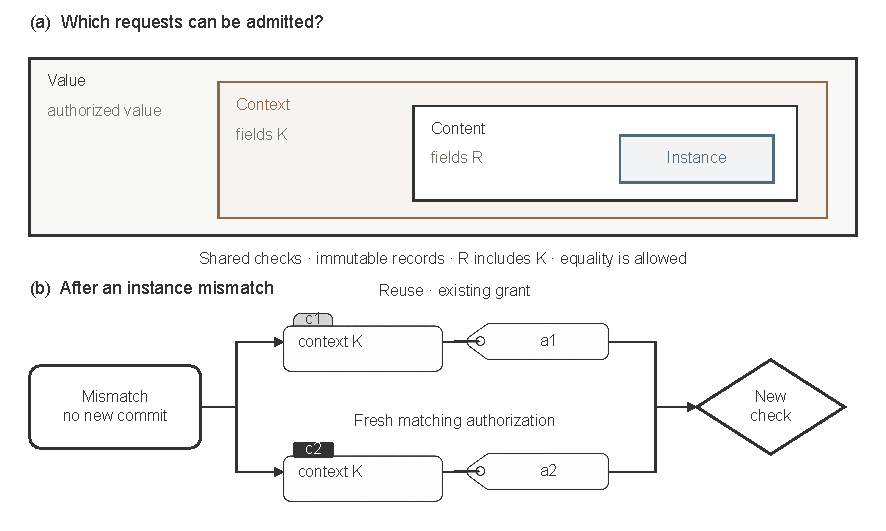
\includegraphics[width=\linewidth]{figures/fig3-design-space.pdf}
\caption{Binding and recovery are separate design choices. Under shared checks and content-immutable candidate records, if the compared content fields \(R\) include the retained context fields \(K\), the admissible request sets satisfy \(A_{\mathrm{instance}}\subseteq A_{\mathrm{content}}\subseteq A_{\mathrm{context}}\subseteq A_{\mathrm{value}}\). These inclusions need not be strict; context and content binding coincide when \(K=R\). Following an instance-mismatch rejection, the system may offer reuse of the reviewed candidate under the existing authorization or obtain matching authorization for another candidate. Reauthorization is a recovery branch, not another binding level. Each continuation must pass a new admission check; the schematic does not guarantee that an available route will be taken. Object glyphs were AI-generated; see the AI-assisted preparation declaration}
\label{fig:design}
\end{figure}

Online Resource 2, A10 maps responsibility rules, compared fields, trusted persistence and continuation to implementation choices. Section~\ref{binding-scope-and-native-defaults} compares three binding rules deterministically; Section~\ref{paired-agent-execution} tests agents under context binding with recorded substitution and instance binding with a continuation channel. The remaining combinations are design options.

GitLab protected-environment deployments must satisfy every configured approval rule. Its deployment-specific approval endpoint accepts \texttt{approved} or \texttt{rejected}, and each user may approve a deployment only once across approver groups \citep{gitlab-deployment-approval}. Redeployment of identical content must satisfy the rules again; merge-request settings separately control vote reset on new commits \citep{gitlab-approvals}. These interfaces establish an operational policy choice, not the prevalence of inappropriate content-scoped approval or unauthorized deployment.

\section{Realization and External Comparison}\label{realization-and-external-comparison}

The relational and event-journal implementations check stored state; a ToolGate adaptation tests whether an existing gate can carry the obligations through its extension interface; and three pinned SDKs determine which reviewed arguments reach execution.

\subsection{Execution gate and independent checks}\label{execution-gate-and-independent-checks}

The contract runs in a relational store and an event journal. The relational adapter reloads state, evidence and authorization within the transaction, validates the principal and unused identities, compares-and-swaps the predecessor, and installs the complete successor, transitions and exact sources. The journal records the same relations under context and exact configurations differing only in instance equality. An independent database oracle reads persisted pre/post relations; a source verifier follows field links through transitions, authorizations, candidates, evidence and predecessors.

The controlled suite runs 165 cases per mechanism. The context journal accepts 60 and rejects 105; the exact journal and relational reference each accept 45 and reject 120. The 15 differences are same-context substitutions. The two exact implementations also agree on provenance-query answers. Request/display probes and the case mapping appear in Online Resource 2, A6.

Bounded formal checks assess the encoded contract. Alloy/Kodkod checks \citep{alloy,kodkod} cover admissions, conjunct removal, source attacks and trace preservation: 72 command outcomes match the manifests, with no assertion counterexamples in the encoded finite scopes. The independent mapping has nine intended satisfiable projections and twenty unsatisfiable mutants (Online Resource 1, S2).

A separate historical audit reconstructs 84 machine-origin correction chains from 1,260 hosted databases. It establishes that the four roles can be recovered from retained persistence records. Per-association and trace counts are reported in Online Resource 2, A5; unchanged-field copying is exercised in the controlled multi-field cases, not these single-field chains (A6).

\subsection{ToolGate implementability case study}\label{configured-toolgate-on-public-reference-workflows}

ToolGate \citep{toolgate} supplies symbolic state and application pre/postconditions. Its normal callbacks express the binding, value, predecessor and source obligations; an author-written SQLite bridge supplies the record schema and durable commit boundary. This tests implementability through extension interfaces, not native default admission.

Execution has four stages: callbacks check the request; the native tool drafts changes in a cloned world; postconditions validate the draft; the bridge installs the successor and its relations in SQLite. Persisted state is then projected back into the public world for the reference suffix (Online Resource 2, A8).

Both implementations pass eight development controls and the shared business and scripted-recovery checks on 24 routes: six pinned tau2-bench Retail workflows \citep{tau2-bench} crossed with four scenarios (Table~\ref{tab:external}). ToolGate's frozen strict failure concerns initialization output, separately retained from business-state scores. Online Resource 2, A8 documents these scripted implementability tests.

\begin{table}[tbp]
\caption{Configured ToolGate ($T$) versus the contract backend ($C$). Development controls and public workflow routes are separate units; decisions and recovery are scripted.}
\label{tab:external}
\centering\small
\begin{tabularx}{\textwidth}{@{}Xrr@{}}
\toprule
Check & $T$ & $C$ \\
\midrule
Development controls satisfied & 8/8 & 8/8 \\
Public: initial authorized business commits & 12/12 & 12/12 \\
Public: invalid requests rejected without a business write & 12/12 & 12/12 \\
Public: fixed legal recovery commits & 12/12 & 12/12 \\
Public: complete reference-world matches & 24/24 & 24/24 \\
Public: frozen strict PASS/FAIL & 23/1 & 24/0 \\
\bottomrule
\end{tabularx}
\par\smallskip
\begin{minipage}{\textwidth}\small
Six public workflows crossed with four controlled scenarios give 24 routes per implementation.
The retained strict failure is two initialization log lines violating an empty-output rule.
Post-hoc inspection confirms that route's business relations and final reference world;
the frozen FAIL is unchanged. Reference-world agreement is not an official benchmark
success rate or evidence of autonomous recovery.
\end{minipage}
\end{table}

\subsection{Binding scope and native defaults}\label{binding-scope-and-native-defaults}

Deterministic probes examine native resume routing, native-to-store composition and binding scope. None calls a model. Online Resource 2, A11 and A14 give the separate protocols, saved runs and reproduction commands.

\textbf{Native human-in-the-loop defaults.} Unmodified LangChain middleware \citep{langchain-hitl} and LangGraph interrupts (versions 1.2.10 and 1.0.8) are tested in author-written graphs, executors and recorders. Sixteen conditions record 18 SQLite effects. Across two turns on the same graph, checkpointer and thread, the old interrupt identifier leaves the new review pending without writing; the current identifier permits one write. A repeated affirmative input at the new interrupt is fresh approval. An explicit edit from 100 to 999 persists 999, preserving the original proposal in checkpoint history; malformed middleware decisions fail without writing. These routes show approval of the pending interrupt, not reuse of an earlier approval for a later request. Same-identifier pending-call replacement and Loopjacking's Agent Server configurations are outside this probe \citep{kumar2026loopjacking}.

\textbf{Reviewed-argument delivery across a restart.} Three separately frozen checks in Online Resource 2, A17 test Agno 3.1.10, LangChain 1.4.7 with LangGraph 1.2.16, and Pydantic AI 2.60.0 (Table~\ref{tab:sdk-checks}). Of 504 constructed cells supplied with complete reviewed per-call objects, 444 match the expected effect multiset. All 84 cells per lifecycle match for LangChain and Pydantic AI, as do Agno's 84 fresh-process cells. Agno's original in-memory run-object route executes another pending call's reviewed arguments in 60 of 72 multi-call cells, reproducing documented issue \#8546.

In a 54-cell ablation, the run-identifier route matches all 18 cells both in process and after a clean restart; the original-object route matches six single-call cells and mismatches all twelve multi-call cells. This implicates the continuation route and its state, while entrypoint and object aliasing change together.

A separate 16-cell check keeps the native call identifier fixed: approval without re-supplying the reviewed object executes substituted arguments in all four cells modifying the supplied message history. Native override executes the reviewed object in all eight override cells, including six substitutions and two unchanged controls. Client-supplied history is a documented application-maintained trust boundary \citep{pydantic-ai-docs}; this result does not identify a framework defect.

\begin{table}[htbp]
\centering\small
\caption{Native-{SDK} checks in Online Resource~2, A17. Constructed cells; the three checks are separate frozen collections scored by the same effect oracle}
\label{tab:sdk-checks}
\begin{tabularx}{\textwidth}{@{}>{\raggedright\arraybackslash}p{0.19\textwidth}>{\raggedright\arraybackslash}p{0.07\textwidth}>{\raggedright\arraybackslash}X>{\raggedright\arraybackslash}p{0.31\textwidth}@{}}
\toprule
Check & Cells & Controlled contrast & Observed outcome \\
\midrule
Reviewed-argument delivery & 504 & Three {SDK}s $\times$ two lifecycles $\times$ seven call scenarios $\times$ six review edits $\times$ two payload families & 444 exact matches; the Agno in-process multi-call cells share the later call's reviewed values \\
Continuation route & 54 & Original in-memory run object; run-identifier route in the same process; run-identifier route after a clean restart & Run-identifier route matches 18/18 in both lifecycles; original-object route matches 6/18 \\
Reviewed-instance substitution & 16 & Identifier-only approval versus override with the reviewed object; substitute the supplied history, the deferred request object or both & Identifier-only approval executes substituted history arguments (4/4); override executes the reviewed object (8/8) \\
\bottomrule
\end{tabularx}
\end{table}

\textbf{Native-to-store composition.} A further scripted graph connects LangGraph 1.0.8 review/resume to the unchanged relational gate and recovery within one in-process execution. Ten conditions cover correction, denial, identity substitution with reuse or fresh review, wrong values, stale predecessors, two rollback points and native/application replay. Both frozen executions satisfy all ten conditions. Per execution, eight authorized corrections commit, while six invalid or rolled-back attempts leave no partial transactional rows; the stale case preserves an independent update. An old interrupt identifier cannot resume the replacement's fresh review. Direct SQL readback checks the candidate, authorization, transition and unchanged-field source relations. This establishes deterministic composition for the tested paths. The trusted adapter registers candidates and creates pre-commit grant handles; the relational gate persists accepted authorization and transition relations atomically. Grant handles and checkpoints remain in process, and decisions are scripted (Online Resource 2, A14).

\textbf{Binding scope.} Nine constructed cases cross three binding comparators and a diagnostic variant with two execution modes, giving 72 routes (54 principal, 18 diagnostic). All arms apply the same request-value guard and differ only in the compared fields (Table~\ref{tab:binding-scope}). In one case the reviewed document changes after review while the candidate stays identical, and a matched control leaves it unchanged. An unchecked executor reads the live document; a verifying executor checks the reviewed digest and consumes the same captured bytes, stopping on mismatch. An independent scorer reads only the persisted effects and compares them with the approved effects saved before execution; it detects deliberate deletion, addition and alteration in copies of each sink.

This experiment uses an extended candidate schema: $K$ contains the target record, operation, unit, source-document digest and proposal; $R$ adds effective date and cost center. A note enters both projections only when declared semantic. Monetary values are normalized to two decimal places. These comparators and the common executor test binding scope, not the full shared gate $G$. In contrast, the contract's declared tuple and the queued-handoff agent experiment use $K=R$ with canonical JSON equality.

% Generated by scripts/figures/build_binding_matrix.py
% FIGURE-DATA.json SHA256: 3a639de0cbd7b11b757ccb84f788dfef3c21ade0fdf660ecaec4792bb0fab6c5
\begin{table}[tbp]
\caption{Binding-gate decisions over nine constructed cases. A: admit; R: reject. Each decision is identical under unchecked and verified execution (72 routes); entries do not report writes. All comparators share the request-value check.}\label{tab:binding-scope}
\centering\footnotesize
\setlength{\tabcolsep}{3pt}
\renewcommand{\arraystretch}{1.12}
\begin{tabularx}{\textwidth}{@{}>{\raggedright\arraybackslash}p{0.46\textwidth}*{4}{>{\centering\arraybackslash}X}@{}}
\toprule
Case & Context & Content & Instance & \shortstack{Raw content\\(diagnostic)} \\
\midrule
% C1-identical-new-instance
C1: Identical new instance & A & A & R & A \\
% C2-effective-date
C2: Effective-date change\textsuperscript{a} & A & R & R & R \\
% C2-cost-center
C2: Cost-center change\textsuperscript{a} & A & R & R & R \\
% C2-effective-date-render-noise
C2: Date change + render noise\textsuperscript{a} & A & R & R & R \\
% C3-referent-mutated
C3: Changed external document\textsuperscript{b} & A & A & A & A \\
% C4-representation
C4: Number/string representation & A & A & R & R \\
% C4-note-display
C4: Display-only note & A & A & R & A \\
% C4-note-semantic
C4: Semantic note & R & R & R & R \\
% C3-referent-unchanged-control
C3: Unchanged-document control\textsuperscript{b} & A & A & A & A \\

\bottomrule
\end{tabularx}
\par\smallskip
\begin{minipage}{\textwidth}\footnotesize\raggedright
\textsuperscript{a}These three changes affect fields omitted from the context key. Context admission produces semantic-violating writes under both executors; content and instance binding reject them.\par
\textsuperscript{b}The reviewed and submitted request values both remain 101.00, so every binding admits. The changed document supplies 999.00 to unchecked execution, which writes it; verified execution blocks the write. The unchanged-document control writes 101.00. This request-value guard is not the full contract's P3 check on the committed value, which would reject 999.00.\par
Raw content omits money normalization and is diagnostic. A note is compared when the case declares it semantic.
\end{minipage}
\end{table}

Context binding admits three changes to the omitted effective-date or cost-center fields; checking the external document's digest does not cover those fields. Content binding rejects the changes through field equality. Instance binding rejects them because each immutable-record change creates a new identifier, avoiding field enumeration in the reuse key. It also rejects three same-semantics re-materializations admitted by content binding: an identical new instance, representation change and display-only note. Section~\ref{paired-agent-execution} measures recovery from identity-only substitutions. The changed-document case passes all four bindings because the candidate is unchanged: the unchecked executor writes the changed amount, the verifying executor writes nothing, and both write the reviewed amount in the unchanged control. Referent protection comes from the executor's consumption check.

\section{Paired Agent Execution}\label{paired-agent-execution}

Once a candidate is rejected, the agent can reuse the reviewed instance, obtain matching authorization, or stop when no route remains. Paired continuations make each choice observable and record the interactions it requires.

\subsection{Design and measurement}\label{design-and-measurement}

Both policies run from the same review checkpoint, so the instance conjunct is the only difference between paired arms. The original study freezes 128 tasks across two provider configurations and two policies: 512 planned arms, one realization per cell. The six families are legal continuation (L, 32), refreshed preview (N, 32), queued handoff (G, 16), changed evidence (E, 16), stale predecessor (V, 16) and receipt unavailability (R, 16). In both collections, all families share an initial instruction not to treat a preview candidate as automatically authorized; N additionally states that a preview does not itself authorize a commit. A deterministic reviewer creates a shared authorization; any candidate that passes validity checking is granted immediately, and a fresh authorization supersedes earlier grants. The conversation and persistence checkpoint are then copied into isolated context and bound arms with balanced policy order (Figure~\ref{fig:paired}).

\begin{figure}[tbp]
\centering
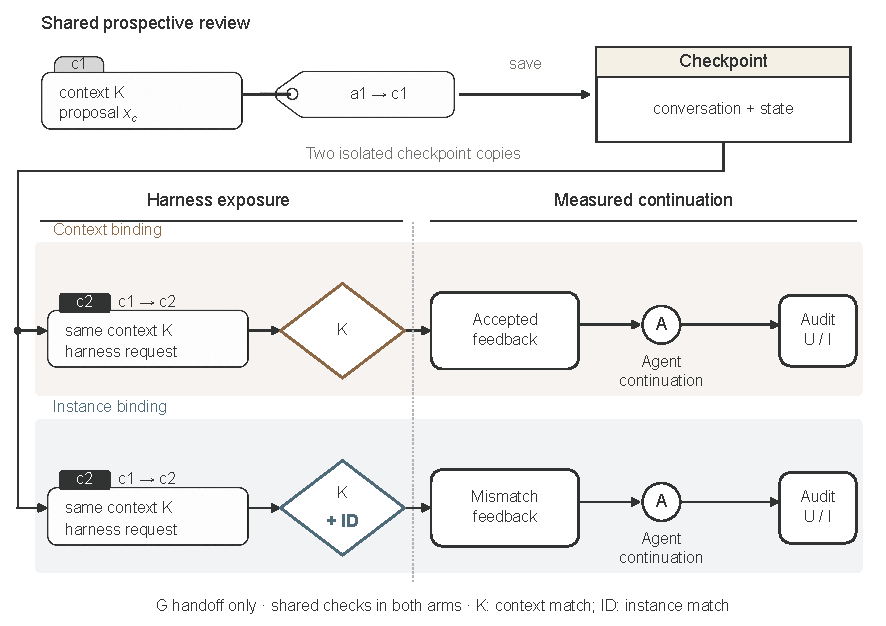
\includegraphics[width=\linewidth]{figures/fig4-paired-intervention.pdf}
\caption{At standardized G handoffs, paired gates differ only in instance equality. The reviewed candidate c1 and its authorization a1 are saved with the conversation and state, then copied into two isolated, directly labelled policy arms. The harness submits c2 with the same context and a different identifier. K denotes $K_{\mathrm{eq}}$; the instance gate adds ID, denoting $I_{\mathrm{eq}}$, while all other checks are shared. Both admission and rejection produce actual feedback for the next sampled agent decision (A), followed by an independent $U/I$ audit. A rejected request makes no commit but leaves the continuation active; subsequent requests must still pass their arm's gate. Measured G outcomes cover 32 delivered pairs from 16 task definitions. N leaves preview management to the agent and is not depicted. Object glyphs were AI-generated; see the AI-assisted preparation declaration}
\label{fig:paired}
\end{figure}

At the queued handoff (G), the harness submits a standardized context-equivalent substitute, after which actual gate feedback enters the next agent decision. The refreshed-preview family (N) leaves management of a required refreshed preview to the agent. Receipt unavailability (R) makes the first receipt query unavailable after a successful commit response has already been delivered; it covers only this confirmed-commit path, and unknown-outcome recovery is a separate deterministic probe (Online Resource 2, A3).

The design separates exposure from behavior. At G, the harness creates and submits the substitute; context admission and the resulting \(I=0\) follow from the policy and oracle definitions, so the 17 and 15 substitution counts are exposure counts rather than agent actions. The harness has already executed the context-side commit when continuation begins; the bound side must recover from rejection. The cost contrast includes this required work. Behavioral observations begin with delivered feedback: whether context arms complete, which legal route bound arms choose, their action sequence through the first persistent recovery commit, and any subsequent confirmation calls.

The online host is a separate reduced implementation shared by A and B, not the relational gate of Section~\ref{realization-and-external-comparison}. Tasks commit one field and record its source as the successor transition identifier, exercising reduced P5/P6. Controlled implementations test multi-field successors, deep source chains and the full evidence graph. With deterministic grants for valid candidates, reauthorization measures agent routing rather than human review burden.

Configuration A requests \texttt{gpt-5.6-terra} through Codex CLI 0.160.1 with low reasoning; no returned model identifier is exposed. B requests and receives \texttt{deepseek-v4-flash} through an Anthropic-compatible Messages API at temperature zero. Both use the same execution system. Each suffix permits 20 decisions and 24 tool calls, with a 90-second request timeout and a 720-second suffix limit. One format-repair allowance applies across the full prefix-plus-suffix history. B has a 4,096-token response cap; A's upstream cap is unavailable. Frozen inputs and complete settings are in Online Resource 1.

\textbf{Collection provenance.} A provider quota prevented 117 original A pairs from receiving any model response before review. Those previously unexposed pairs form a separately frozen supplementary A collection of 234 arms, retaining task definitions, prompts, tools, policy ordering, requested configuration and scoring. Original outcomes remain unchanged; the later, selected collection has its own denominator and exploratory analysis.

The independent oracle scores utility \(U\) from authoritative goal attainment, required workflow and accurate final reporting. Integrity \(I\) is 1 with sufficient coverage and no contract violation. A proved violation yields 0, and incomplete necessary evidence yields unknown unless a violation is already proved. With no authoritative transition, integrity can hold vacuously and carries no evidence about contract conformance. The instance-continuity oracle applies to both policies, so a context-admissible substitution can score \(I=0\): \(I=0\) records non-conformance to the declared instance rule, not a safety failure under the context rule that the arm declares. Admissibility under a policy and conformity to the independent oracle are different judgments.

For aggregate completion differences, each task contributes the mean of its configuration-specific paired differences (bound minus context). We bootstrap 128 task clusters within family, retaining both policies and configurations (10,000 iterations, seed 20261007). We apply the same procedure separately to the 117 supplementary pairs. Recovery summaries condition on feedback in a saved model input followed by a received response. Recovery calls run from that feedback through the first successful commit that adds a persistent transition; subsequent calls are counted separately. Complete-suffix cost remains the bound-minus-context difference over both full continuations.

\subsection{Task completion and instance continuity}\label{continuity-and-task-completion}

Substitutions that context binding admits mostly complete their tasks. All proved substitutions occur at G under context binding: 17 in the original collection and 15 in supplementary A. Thirty of these 32 arms still complete their task, so an audit of endpoint utility alone would classify them as successful; the continuity oracle separates them. The 32 episodes come from 16 G task definitions, each observed under deployments B and A. The corresponding bound arms reject the substituted request and all finish with \(U=1,I=1\). Table~\ref{tab:outcomes} retains complete cohort denominators, including quota failures and unknown integrity; family-level joint outcomes are in Online Resource 1, S11--S12.

\begin{table}[tbp]
\caption{Completion and instance substitution by collection. Context (Ctx) and instance (Inst; archived as bound) counts are separate; completion denominators remain the planned pairs.}\label{tab:outcomes}
\centering\small
\setlength{\tabcolsep}{2pt}
\begin{tabular*}{\textwidth}{@{\extracolsep{\fill}}lrrrrrrrr@{}}
\toprule
Collection & \shortstack{Planned\\pairs} & \shortstack{Verified\\checkpoints} & \multicolumn{2}{c}{Completion} & \multicolumn{2}{c}{Substitutions} & \multicolumn{2}{c}{$I$ unknown} \\
\cmidrule(lr){4-5}\cmidrule(lr){6-7}\cmidrule(lr){8-9}
 & & & Ctx & Inst & Ctx & Inst & Ctx & Inst \\
\midrule
Original A & 128 & 11 & 9 & 9 & 1 & 0 & 0 & 0 \\
Original B & 128 & 128\textsuperscript{a} & 117 & 119 & 16 & 0 & 1 & 1 \\
Supplementary A & 117 & 117 & 114 & 116 & 15 & 0 & 0 & 0 \\
\bottomrule
\end{tabular*}
\par\smallskip\begin{minipage}{\textwidth}\small Planned pairs are also planned arms per policy; both policies together double that count. Checkpoints count verified prefix events and matching saved states. Original A includes 117 pairs stopped by quota before review; supplementary A evaluates those pairs later. \textsuperscript{a}All 128 original-B pairs reached review, but only 127 pair-summary flags survive. N-020-B has a saved checkpoint event and state; its context suffix is partial and its bound suffix was not started. These two integrity scores remain unknown. $I$ denotes instance-rule conformance; no-transition arms can satisfy it vacuously.\end{minipage}
\end{table}

Planned-ledger completion includes pre-review service failures. Original B completes 117/128 context and 119/128 bound arms (+1.56 percentage points; 95\% task-cluster interval {[}−3.91, 7.03{]}). Original A completes 9/128 under each policy with no discordance. The pooled 126/256 versus 128/256 contrast and interval are therefore exactly half the B values: +0.78 points {[}−1.95, 3.52{]}. This is a denominator rescaling of the same discordance, not additional precision. The supplementary difference is +1.71 points {[}0.00, 4.27{]}. Neither comparison establishes a completion advantage (Section~\ref{threats-to-validity}). Original B has 18 capped invalid-output terminations (10 context, 8 bound), including two G context arms; this imbalance constrains interpretation of the original-B completion difference.

A later 24-task output-budget check gives context/bound completion of 23/24 versus 22/24 at 4,096 tokens, and 24/24 for both at 393,216 tokens. Integrity remains 20/24 versus 24/24 at both caps, including four programmed context substitutions per cap. This 96-continuation study uses a later collection period and longer waits; its full results and the original failure decomposition are in Online Resource 2, A1--A2.

\subsection{Two routes to recovery and their cost}\label{two-routes-to-accountable-recovery}

All 32 delivered G-bound mismatches recover. Original B's 16 continuations reuse the reviewed candidate; supplementary A has eight reuse and seven reauthorization paths; original A's single mismatch also uses reauthorization. Agents thus select different legal continuations under the same admission rule (Figure~\ref{fig:recovery}).

\begin{figure}[tbp]
\centering
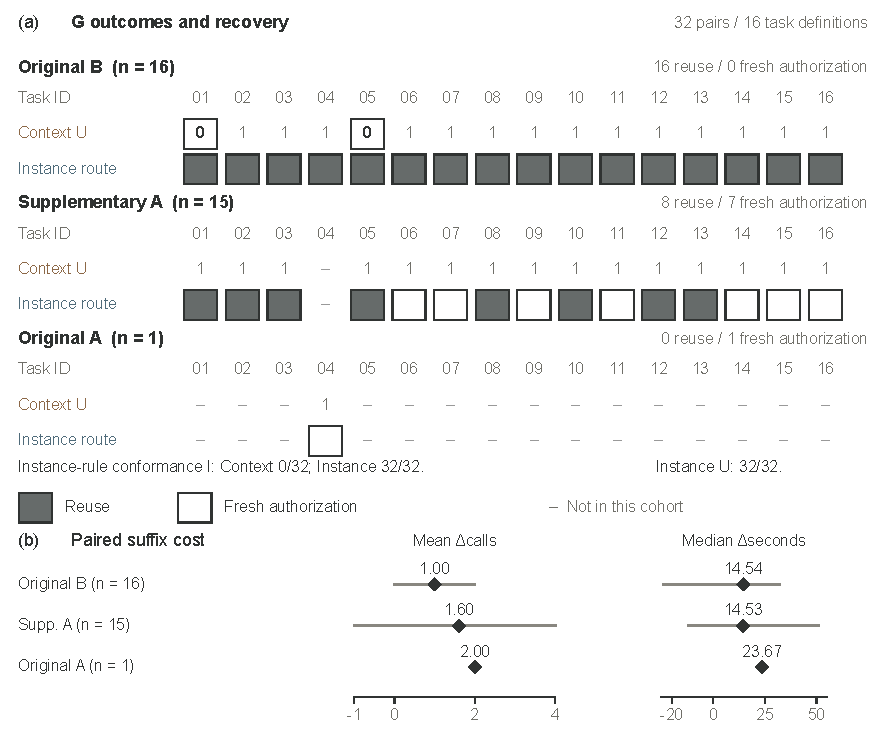
\includegraphics[width=\linewidth]{figures/fig5-recovery-cost.pdf}
\caption{All 32 delivered G pairs across 16 task definitions. (a) Task columns align across cohorts; dashes mean absent from that cohort's delivered pairs, not failure. Supplementary A omits 04; Original A includes only 04. $I$ denotes instance-rule conformance, not safety under the context policy. Context has $I=0$ throughout and $U=1$ in 30 pairs; all bound arms end with $U=1,I=1$. Filled/open squares denote reuse/fresh authorization. (b) Diamonds show mean call and median elapsed-time differences for complete paired suffixes ($\Delta=$ bound minus context); segments show observed minima--maxima, not confidence intervals. Time includes decisions, tool interactions and terminal paths. Table~\ref{tab:recovery-decomposition} separates recovery calls}
\label{fig:recovery}
\end{figure}

A post-hoc reconstruction checks whether these choices reflect different available routes. For all 32 episodes, the saved rejection state retains an active original grant, an unchanged reviewed candidate, valid evidence and a current predecessor, and the saved model input contains that candidate, grant and authorized value. These checks use the state and input bytes rather than the host's logged list of legal paths. Reuse was therefore both available and visible at the observed boundary, including in all eight episodes that requested fresh authorization.

After delivered feedback, each of the 24 reuse episodes makes one commit; each of the eight fresh-authorization episodes requests authorization and then commits. No failed or exploratory call intervenes. Later receipt or state queries are separate continuation actions (Table~\ref{tab:recovery-decomposition}); grants are immediate and deterministic. Across the 16 matched task definitions, A and B both reuse in eight; A reauthorizes while B reuses in eight. A combines one original and fifteen later supplementary episodes, so this is a descriptive route contrast, not an identified model effect (Online Resource 2, A12). Online Resource 1, S12.6 illustrates the saved input, recovery commit and subsequent receipt query in one episode.

\begin{table}[tbp]
\caption{Agent tool calls at delivered G handoffs. All entries except $n$ are cohort means; post-commit calls occur after the first successful persistent recovery commit.}\label{tab:recovery-decomposition}
\centering\small
\setlength{\tabcolsep}{3pt}
\begin{tabular*}{\textwidth}{@{\extracolsep{\fill}}lrrrrrr@{}}
\toprule
Collection & $n$ & \shortstack{To recovery\\commit} & \shortstack{After\\commit} & \shortstack{Bound\\suffix} & \shortstack{Context\\suffix} & $\Delta$ \\
\midrule
Original A & 1 & 2.000 & 2.000 & 4.000 & 2.000 & 2.000 \\
Original B & 16 & 1.000 & 0.375 & 1.375 & 0.375 & 1.000 \\
Supplementary A & 15 & 1.467 & 1.533 & 3.000 & 1.400 & 1.600 \\
\bottomrule
\end{tabular*}
\par\smallskip\begin{minipage}{\textwidth}\small Recovery comprises one commit in each of 24 reuse episodes and an authorization request followed by a commit in each of eight fresh-authorization episodes. The last column is bound minus context over complete suffixes, not calls beyond a route minimum. Values are recomputed from the archived event order and persistent transitions; no new runs are added.\end{minipage}
\end{table}

Complete paired suffixes add a mean 1.00 tool call and median 14.54 seconds in original B ($n=16$ pairs), versus 1.60 calls and 14.53 seconds in supplementary A ($n=15$). A new exploratory paired bootstrap gives 95\% intervals of {[}0.75, 1.25{]} and {[}0.87, 2.33{]} calls, respectively; these condition on the constructed task sample (Online Resource 2, A12). The latter's seven reauthorization paths add 0.47 authorization requests per pair; original B adds none. Original A's single pair adds two calls and 23.67 seconds, including one authorization request; no interval is estimated. Full-suffix differences include required recovery, later confirmation and context-side calls; they need not equal route minima. These request counts expose a cost that immediate deterministic grants cannot price: a real workflow may require another review and queue wait. They are not estimates of human time. Table~\ref{tab:recovery-decomposition} separates recovery, subsequent and context-side calls; Figure~\ref{fig:recovery} preserves signed ranges. E/V/R results remain separate in Online Resource 1, S11--S12.

\subsection{Recovery when permission or feedback changes}\label{feedback-sensitivity}

Recovery also depends on current permission, not just candidate identity. A separately frozen exploratory study collected on 14 October 2026 uses four task instances from the same G family, each under three post-rejection states: the old grant remains valid, it is revoked while the reviewer remains available, or the reviewer is unavailable and no legal route remains. Each state compares current permission facts alone with the same facts plus derived legal-path labels. The resulting 12 pairs comprise 24 hosted trajectories using deployment B's requested alias, a 393,216-token output cap and longer waits; 24 deterministic rule trajectories are separate controls. Each cell runs once. Online Resource 2, A13 gives selection, allocation, raw-record audit and reproduction details.

Both feedback variants complete all eight feasible episodes and stop without a write in all four unavailable episodes; all twelve episodes per variant preserve integrity. Each variant uses sixteen tool calls, including four authorization requests, with zero rejected continuation operations. Paired call differences (labels minus facts) are $-1$ in three pairs, zero in six and $+1$ in three. The rule controller also completes feasible episodes and stops in unavailable ones. By permission state, the four paired call differences sum to $+2$ for valid grants, $+1$ for revoked grants and $-3$ when no route remains; the aggregate zero masks this descriptive variation. Secondary totals are lower with labels: 283.751 versus 371.048 seconds and 49,293 versus 66,774 output tokens; A13 retains all state-specific results. These twelve pairs reuse four task definitions. The study shows permission-sensitive continuation but no net tool-call benefit from path labels. It neither establishes feedback equivalence nor supports an LLM-specific advantage. The sample is kept separate from the original completion estimates and the 32 delivered G pairs.

A new dynamic pilot separates availability at feedback from permission at the next commit. Two reused tasks cross four conditions: no change, selected-grant revocation, predecessor advance, and no remaining legal route. All eight hosted first commits were initially admissible; six were correctly rejected after the injected change. Hosted and adaptive-rule controllers both restore all six feasible business states and correctly stop in the two unavailable cases. A cached-route control restores only the two static cases. Independent SQLite readback verifies the effects and final reports. This pilot does not establish an LLM advantage; Online Resource 2, A16 preserves all 24 trajectories and a narrower frozen confirmation metric requiring a matching final \texttt{get\_state} query.

\subsection{Exposure without rejection feedback}\label{opportunity-and-voluntary-behavior}

Agents shown a context-equivalent alternative reused the reviewed instance or obtained fresh authorization. The N family supplies such an alternative without forcing its submission. Across the collections, 186 arms were planned, 185 retain state and 127 reached review. Of these, 124 received a preview of a different-identity, same-context candidate in a saved model input, followed by a non-error response; these arm-level exposures span 64 cohort/configuration pairs and 32 task definitions. Sixty pairs expose both arms and four expose one. Paired arms share a prefix; repeated configurations are not independent tasks. Agents reused the reviewed instance in 123 cases and obtained matching authorization for the previewed candidate in one; there were zero unauthorized substitutions.

One original-B context arm supports only observation through its saved after-state, and its bound counterpart was not started; both integrity scores remain unknown. Excluding the partial arm leaves 126 reviewed arms, 123 exposures, 122 reuses and one reauthorization (Online Resource 2, A7). N thus shows two continuity-preserving behaviors when an alternative is available. G measures recovery from delivered mismatch feedback; N contains no such feedback.

\section{Discussion}\label{discussion}

\subsection{Implications}\label{design-implications}

The evidence is a comparison of scopes and their continuations, not a new enforcement mechanism. Omitted fields, equivalent replacements and mutable referents require different checks; persisted-state and extension tests show where those checks can run. Admission alone does not determine continuation: eight recovered mismatches prompted fresh authorization despite an available, visible grant.

A context-scoped policy that admits an identity-different, content-identical candidate is following its own rule. The continuity oracle records non-conformance to the instance rule, not a safety failure, and the engineering question is which scope an application declares and whether its continuation interface is consistent with that choice.

Because the candidate, grant and authorized value were present in the saved model input, missing information within this fixture cannot explain the eight fresh authorizations. The agent's interpretation of rejection and the offered continuation remain relevant design factors that an admission-only audit misses.

Endpoint-value audits cannot distinguish reviewed artifacts from regenerated equivalents. Approval scope instead requires auditing the relation among candidate, authorization and committed transition.

The exploratory feedback comparison sharpens the interface implication. With the same permission facts, adding path labels produces no net tool-call reduction; when no legal route remains, truthful stopping is the appropriate endpoint. An implementation should expose current authority and the reviewed object, then distinguish recovery, confirmation and renewed review in its telemetry. The evidence does not prescribe a universal route-selection strategy.

Read together, the results make approval scope, the enforced execution boundary and recovery behavior one interdependent design problem, decided at four points:
\begin{enumerate}
\tightlist
\item \textbf{Obtain the responsibility rule.} Have the workflow owner state whether approval covers a value, retained context, declared content or the reviewed artifact, and which replacements may reuse it. The measurements do not decide this organizational requirement.
\item \textbf{Cover the reusable content.} Put each decision-relevant field in the reuse key or check its approved value separately at execution; declare the comparator.
\item \textbf{Anchor binding and recovery.} Resolve identifiers through trusted lookup to immutable candidates; return the reviewed identifier or the state/evidence mismatch needed for reuse or fresh authorization. A valid original grant can support reuse even for an irreversible operation; stale state or evidence can require fresh authorization even for a reversible one.
\item \textbf{Check external objects at consumption.} Verify the reviewed digest and execute on the same captured bytes, as in the binding-scope experiment's verified executor.
\end{enumerate}

ToolGate callbacks and a commit bridge carry the application obligations; the native-to-store experiment checks their composition with interrupt routing, stale state and rollback. Deployment still requires restart-safe grant/checkpoint storage, authenticated review and evaluation with autonomous agents and real approval delays.

\subsection{Threats to validity}\label{threats-to-validity}

\textbf{Construct validity.} Measured costs are agent-side tool calls and suffix time. Gate computation was not isolated; human re-inspection and approval-queue waiting were not measured. The deterministic reviewer immediately grants any valid request, whereas a deployed reauthorization request may wait, be refused or require transfer to an authorized reviewer. The observed routes and suffix times do not establish optimal route selection or production approval latency. Canonical equality is enforced at the gate; agreement between displayed and compared values was tested only in the browser fixture. The binding-scope study implements the selected comparators and a common executor, not the complete set of shared checks \(G\), and normalizes money to two decimals instead of canonical JSON equality.

\textbf{Internal validity.} G substitutions are harness-created exposures (Section~\ref{design-and-measurement}), and each cell has one realization. G recovery and N continuation were observed under the common preview--authorization instruction, with an additional reminder in N; no control without warnings isolates these prompts' effects. The archival availability audit is post-hoc and establishes a saved-state property, not the outcome of an unchosen counterfactual route. The completion comparisons are not powered for a non-inferiority claim, and an interval that includes zero does not establish equivalence. The supplementary cohort and output-budget study retain separate collection conditions and denominators. The feedback comparison uses four previously used task definitions in a separately frozen collection; its paired fact control isolates added labels within that fixture, but not effects of all feedback or differences across collection periods. The deterministic binding protocol was amended after inspecting an initial run, and its 72 routes are crossed conditions over nine constructed cases, not independent samples.

\textbf{External validity.} Constructed tasks, deterministic review and the reduced single-field host leave natural mismatch prevalence, human approval cost and production benefit unmeasured. ToolGate uses scripted decisions and an author-written commit bridge, not native default enforcement or autonomous agents. Native-to-store checkpoints and pre-commit grant handles remain in memory. The separate SDK checks cover clean restarts, continuation routes and controlled substitution of supplied history; they do not test crash recovery, restart-safe application grants, concurrent replay, reviewer authentication or other hostile pending-state mutations. Each SDK result is limited to its pinned version and tested route, not framework-wide safety. Only two design-space points have agent evidence; the remaining combinations lack developer-study validation.

\textbf{Measurement boundary.} The native checks compare executed effects keyed by the runtime tool-call identifier written by the tool body. Recovering the reviewed-call mapping when that identifier itself cannot be trusted is a separate open problem and is not addressed here.

\textbf{Scope of the formal results.} The formal and persistence results apply to the stated local observation model and atomic single-record successor (Section~\ref{what-endpoint-correctness-cannot-establish}); multi-record or distributed enforcement requires additional coordination.

\subsection{Directions for future work}\label{future-work}

Four directions follow from the boundaries above. Recovering the reviewed-call mapping when the runtime call identifier cannot be trusted is a separate open problem: it needs either a trustworthy execution identifier or an independent record of what the tool body executed. Restart-safe and concurrently enforced authorization state, reviewer authentication and hostile mutation of pending state are untested here, and each matters once approval leaves a single in-process host. Replacing the deterministic reviewer with a production approval queue would measure human approval latency and the real cost of renewed authorization. Finally, only two points of the design space have agent evidence; developer studies of the remaining combinations, and of multi-record or distributed enforcement, would show how far the contract extends.

\section{Conclusion}\label{conclusion}

An approval's binding object determines which replacements it permits. That is an admission decision; how an agent recovers after a rejection is a separate, observable choice. The four-role correction contract connects the admission choice to authorized values, successor structure and field sources. The tested agents recover from all delivered identity-only rejections when the original grant remains usable and present in model input, yet sometimes request new authorization. The exploratory permission-state study also demonstrates stopping when no legal route remains, with no net tool-call reduction from additional path labels in this sample. The practical implication is to enforce a declared approval scope and to measure its continuation, including authorization requests whose human-review costs remain unmeasured.
\section*{Statements and Declarations}
\subsection*{Data and software availability}
Constructed tasks and archived review checkpoints underpin the study. Frozen archives retain the controlled experiments at commit \href{https://github.com/lhh666-6/auto-dete/tree/2645e5e18c900ea91c9c980e44195dc71e410432/DKE-supplement}{\nolinkurl{2645e5e18c900ea91c9c980e44195dc71e410432}}, and the reference implementation, formal models and earlier historical evidence at \href{https://github.com/lhh666-6/auto-dete/tree/c6d512843c905cab6d8521dd8c914f7fb26d85ae/latest}{\nolinkurl{c6d512843c905cab6d8521dd8c914f7fb26d85ae}}. The prospective inputs and runner have master-manifest SHA-256 \nolinkurl{7773563b40c8db30d6def121915f50fbad032537edde32afd4ba39ec3eea744b}. The handoff archive at \href{https://github.com/lhh666-6/auto-dete/tree/475e66f549613aaaaa62c2ec81ffdee483636c54/cloud-handoff}{\nolinkurl{475e66f549613aaaaa62c2ec81ffdee483636c54}} contains the complete original ledger, responses, states, scorer, tables, figure sources and hashes (Online Resource 1). Supplementary A retains its separate freeze, complete attempts, independent scores and source hashes, with the offline entry point in S12. The pinned \href{https://github.com/lhh666-6/auto-dete/blob/f5fe7231c5e808ba1629132d222f448bff471204/REPRODUCIBILITY.md}{reproduction guide} orders the offline workflow. Reanalysis needs no model calls; new hosted runs require provider access.

{\urlstyle{tt}\nolinkurl{X1-X2-reproduction.zip}} contains versioned sources, two saved executions and independent offline SQLite verification for native approval and binding scope (Online Resource 2, A11). A17 documents three separate archives: {\urlstyle{tt}\nolinkurl{Correction-consumption-reproduction.zip}} (504 cells), {\urlstyle{tt}\nolinkurl{Agno-entrypoint-reproduction.zip}} (54) and {\urlstyle{tt}\nolinkurl{Reviewed-instance-substitution-reproduction.zip}} (16). These retain frozen protocols, code, cases, source/SDK seals, raw per-cell effects, scores, reports and portable offline verifiers; the first also retains adapter and scoring reviews.

{\urlstyle{tt}\nolinkurl{Native-contract-reproduction.zip}} retains the scripted native-to-store source freeze, unchanged backend dependencies, two saved runs, independent SQL scorer and negative controls (Online Resource 2, A14); it calls no hosted model.

The source package supplies recovery-cost readback and hashes, an anchored example, availability reconstruction for all 32 G pairs, and Table~\ref{tab:recovery-decomposition} recomputation. \texttt{REPRODUCE-RECOVERY.md} lists the two archive dependencies, hashes and offline commands; \texttt{--output} separates derived files. These analyses add no runs. {\urlstyle{tt}\nolinkurl{Feedback-sensitivity-reproduction.zip}} supplies the frozen exploratory study, raw trajectories, dependencies and read-only instructions in \texttt{REPRODUCE.md}. {\urlstyle{tt}\nolinkurl{Dynamic-recovery-reproduction.zip}} contains the pilot protocol, eight hosted trajectories, sixteen rule controls, independent scoring and offline replay. Original and supplementary ledgers remain separate.

\subsection*{Ethics approval and consent to participate}
The prospective experiment uses constructed tasks and a deterministic host reviewer, with no new human participants. In the historical annotation study, one author (X.W.) and one non-author volunteer independently coded benign completion outcomes; L.H. adjudicated their single inter-coder disagreement and separately reviewed eleven cases in which the strict trajectory label and the endpoint rule disagreed; a separate textual-acknowledgment audit with 39 human--rule disagreements was not adjudicated and is reported only as human--rule agreement. X.W. also completed the textual-acknowledgment annotation. Only pseudonymous annotator identifiers were collected. Both coders were informed of the task and data use, and the non-author coder participated voluntarily. The authors assessed the annotation of generated outputs as not requiring ethics approval. Online Resource 1, S5.2 details the annotation procedure. No animal subjects were involved.

\subsection*{Consent for publication}
Not applicable; no identifiable participant information is reported.

\subsection*{CRediT authorship contribution statement}
Liang Hanghao: Conceptualization, Methodology, Software, Formal analysis, Investigation, Data curation, Validation, Visualization, Project administration, Writing--original draft, and Writing--review \& editing. Xuan Wentao: Methodology, Formal analysis, Investigation, Data curation, Validation, Visualization, and Writing--review \& editing. Chen Qile: Investigation and Validation. Peng Peng: Supervision and Writing--review \& editing.

\subsection*{Funding and competing interests}
This research received no external funding. The authors declare no competing interests.

\subsection*{AI-assisted preparation}
ChatGPT 6 Astra assisted with language polishing and selected experimental verification tasks. Codex assisted with auditing experimental procedures and results, developing research code and verification scripts, and manuscript editing.

Illustrative object glyphs in Figs.~\ref{fig:gap}--\ref{fig:paired} were generated on 21 October 2026 using OpenAI's built-in image-generation tool from author-defined specifications. The diagrams were assembled in code, with labels, values and connections set separately. The underlying image-model version was not provided by the interface. The supplied figure sources retain the specifications, original assets and placement code.

The authors retain full responsibility for the research design, analysis, interpretation and final manuscript.

\subsection*{Supplementary information}
Online Resource 1 contains formal checks, workloads, historical records, prospective definitions, complete outcomes and the artifact map. Online Resource 2 contains supplementary experiments and audits (A1--A8), extended specification and design guidance (A9--A10), native approval and binding scope (A11), recovery availability and feedback (A12--A13), native-to-store composition (A14), obligation foundations (A15), dynamic recovery (A16) and the three native-SDK checks (A17). Online Resource 3 collects the editable sources and seven reproduction archives described above. Original and supplementary ledgers remain separate.

\bibliography{references}
\end{document}
